\appendix
\label{appendix_start}
\chapter{Interviews}
  \label{chap:interviews}
Interview resultater med forbigående fodgængere og cyklister ved Nytorv/Østerågade i Aalborg I dette afsnit er 4 spørgsmål beskrevet, som blev stillet og svarerende fra 20 forbigående fodgængere og cykelister ved Nytorv/Østerågade, hvor de væsentlige svar er med i rapporten.
~\\
  \textbf{Spørgsmål 1.}
  Føler du dig tryg ved, at gå over fodgængerfeltet, når der er mange cyklister ude ved Nytorv/Østerågade i Aalborg?
~\\\\
  \textbf{Svar 1.} ~\\
 \emph{”Jeg føler mig tryg af, at gå over fodgængerfeltet, når der er mange cyklister. Jeg synes at de fleste holder pænt tilbage”.}
~\\\\
  \emph{”Jeg er Københavner, og jeg synes, at det er mere betryggende, at gå ude på strøget i København, der cykler ingen forbi, der er kun tværgående trafik. Jeg synes, at det er værre med bilerne, også må cyklisterne gerne være herude synes jeg.”}
~\\\\
  \emph{”Jeg bruger normalt lidt tid på, at se efter om cyklisterne har set mig eller om jeg selv skal stå tilbage, også går jeg over”}
~\\\\
\emph{” Jeg synes godt, at der kan være kaos herude nogle gange, og det er både cyklister, biler og busser der skaber den kaos.”}
~\\\\
  \emph{”Jeg føler mig tryg, da jeg tror at cyklisterne tænker, at jeg er gammel og de skal passe lidt på, men jeg træder aldrig ud uden at se mig for, jeg passer virkelig på.”}
~\\\\
  \emph{“Nej - holder øje til højre og venstre, og så kommer der nogle gange også en bil som ikke skal køre herinde.”}
~\\\\
  \emph{“Jeg føler mig tryg og cyklerne holder tilbage for en.”}
~\\\\
  \emph{“Nej - cyklerne holder ikke færdselsloven og holder ikke tilbage for fodgængerne.”}
~\\\\
  \emph{“Jeg føler mig tryg, når jeg går over vejen. En gang imellem ser man, at nogle stopper op og andre gør ikke, men jeg har ikke noget problem med det.”}
~\\\\
  \emph{“Ja det er jeg - de er gode til at holde tilbage.”}
~\\\\
  \emph{“Egentlig ikke - jeg synes, at cyklerne kommer meget uventet og meget hurtigt. Jeg holder utroligt meget øje.”}
~\\\\
\emph{“Nej egentlig ikke - de holder ikke tilbage - det er cyklerne- jeg er mere tryg ved bilerne.”}
~\\\\
\emph{“Ja det gør jeg faktisk - der er mange mennesker, men jeg synes ikke det er et problem.”}
~\\\\
  \emph{“Ikke altid - jeg er lige hoppet over for en cyklist.”}
~\\\\
  \emph{”Jeg bor lige herude. Man kan ikke gå og regne med at der ikke er andre end en selv herude, men jeg synes ikke engang at der er ret trafikeret, det kunne have været meget værre. Jeg synes at det er helt fint herude.”}
~\\\\
  \emph{“Cyklisterne kører sgu som en brækket arm, Så nej jeg føler mig ikke tryg.”}
~\\\\
  \textbf{Spørgsmål 2}
  ~\\
  Hvad er det, der gør dig utryg/tryg, når du går over fodgængerfeltet? og hvad er det vigtigste for dig, for at du føler dig tryg i et integreret trafikmiljø?
~\\
  \textbf{Svar 2} ~\\
\emph{“Noget mere overvågning, så biler der ikke skal køre derinde, ikke kan komme ind.”}
~\\\\
  \emph{”at vi fodgængere, cyklister og biler nærmest deler vejen, og at det ikke alle der tager hensyn til hinanden, vil føle mig mere tryg hvis vi var delt.”}
~\\\\
  \emph{“Her på Boulevarden lagde jeg mærke til at cyklisterne ikke kunne være der, så de måtte trække deres cykler på fortovet. De kunne slet ikke være der overhovedet.  Derfor stiller jeg min cykel i Arkaden og går hernede.”}
~\\\\
  \emph{“Jeg benytter mig af fodgængerovergangen, og det gør mig tryg.”}
~\\\\
  \emph{“At færdselsloven bliver overholdt.”}
~\\\\
  \emph{“Det må være det, men om morgenen så er der fart på her i området, altså mange folk cykler mod skoler, universitet og på arbejde. Men så længe at vi alle opmærksomme og buschaufførerne ved godt, at der er fodgængere her, så de er også opmærksomme, at området er gågade.”}
~\\\\
  \emph{“At folk viser hensyn til hinanden.”}
~\\\\
  \emph{“Folk holder automatisk tilbage - det gør de jo ikke.”}
~\\\\
  \emph{“At fodgængerfeltet er helligt og folk holder tilbage.”}
~\\\\
  \emph{“Det er at busserne og bilerne holder tilbage. Det er dem der kan lave noget skade. Jeg har gået herinde rigtig meget, og jeg har aldrig set en ulykke.”}
~\\\\
  \emph{“At jeg kan gå over, når jeg synes der er fri bane.”}
~\\\\
  \emph{“Man ved aldrig om cyklerne holder tilbage.”}
  ~\\
  \textbf{Spørgsmål 3}
  ~\\
  Har du nogle ønsker eller forslag til, hvordan man kan binde gågaden sammen?
~\\
  \textbf{Svar 3} ~\\
  \emph{”Man kan ikke se fodgængerfeltet, det er ikke tydeligt nok i den grå farve. Jeg synes godt, at man kan male fodgængerfeltet hvidt.”}
~\\\\
\emph{“Jeg synes bilerne skal fjernes herfra, men busserne er okay.”
  ”Jeg synes godt, at man kan lave en bilfrizone herude, og lave flere cykelstier, med nogle gennemveje.”}
~\\\\

  \emph{”man kunne evt. lave en undergang eller overgang.”}
~\\\\
  \emph{“Det er bare fjerne alt trafikken herinde på Nytorv. Det er ganske enkelt.”}
~\\\\
  \emph{”Man kunne evt. dele os mere op, så bilerne havde deres egen kørebane og cyklisterne havde en cykelsti, de kunne cykle på.”}
~\\\\
  \emph{“Jeg ved ikke om det er praktisk, men man kunne jo bygge en gangbro, i stedet for de fodgængere felt, men hvis man ser på højden af busserne, så ved jeg ikke om det er realistisk. Ellers så vil mit bud være, at lave en tunnel, som man har ved Aalborg banegård.”}
~\\
\textbf{Spørgsmål 4}
~\\
Hvad synes du om, at lave en cykelsti uden om Nytorv og derved udelukke cyklisterne helt fra området?

~\\\\
~\textbf{Svar 4} ~\\
\emph{”jeg synes ikke, at man skal udelukke cyklisterne fra Nytorv, jeg synes mere at man skal udelukke privatkørsel på en eller anden måde.”}
~\\\\
  \emph{“Jeg ved, at butikkerne er imod, at man lukker for trafikken her i Nytorv, da de mener at deres salg vil gå ned. Men det passer altså ikke, fordi der er et gammelt universitets undersøgelse der har vist, fluger tror jeg, at det faktisk vil gå bedre hvis der kun er gågade. De vil sælge mere.”}
~\\\\
\emph{”Jeg kommer oprindeligt fra Kina, og der synes jeg ikke at det er et problem, med at dele trafikken, busserne, bilerne og cyklisterne holder pænt, derfor synes jeg ikke at man behøver, at udelukke dem fra Nytorv."}
~\\\\
\emph{ “Jeg tror de vil blive ret sur, fordi der mange der kører gennem midtbyen her. Men jeg tror heller ikke man kan gøre det. Hvis man ser på større byer, som København og Aarhus, hvor cyklister er integreret del af bylivets trafik, så det vil ikke være umuligt.”
  ”jeg synes ikke, at man skal udelukke cyklisterne fra Nytorv.”}
~\\\\

  \emph{“Ja, bare ikke begge ender. Det vil skabe bedre vækst for butikkerne og bedre sikkerhed for fodgængere i området.”}
~\\\\
  \emph{”jeg synes, at det vil være i orden, at udelukke cyklister fra Nytorv, så man var delt.”}
~\\\\
  \emph{“Jeg tror ikke det vil hjælpe at lede en cykelsti uden om Nytorv, da cyklerne bare vil cykle derinde alligevel. Jeg tror derimod det vil hjælpe at sætte nogle bump op, så det kun er erhvervsbiler der kan køre herinde.”}
~\\\\
  \emph{“Det vil være en drøm at gøre Nytorv cykel-, bil- og bus-frit.”}
~\\\\
  \emph{“Det lyder som en god ide, at lede cyklerne uden om Nytorv eller dele cyklisterne ud fra kørebanen, så de fik en cykelsti. ”
  “Det vil være fint at udelukke bilerne, men cyklerne synes jeg ikke. Det giver lidt liv, og de skal også frem og tilbage, og det skal der også være plads til.”}
~\\\\

  \emph{“Jeg synes det vil være en god ide at udelukke bilerne herfra, men ikke cyklerne. Bilerne skaber et kaos.”}
~\\\\
\emph{“Jeg synes ikke cyklerne skal ledes uden om Nytorv, for det er rimelig praktisk pga der er mange handelsmuligheder osv. Men jeg synes der skal noget bedre markering på vejene.”}
~\\\\
\emph{“Det ved jeg næsten ikke, hvordan det skal laves. Måske busserne og bilerne, men der er meget der skal undersøges, for der er mange stoppesteder hernede.}

\chapter{ÅDT udregninger}
  \label{chap:aadtregninger}
  Bemærk at, AA er det samme som Å, eftersom LaTeX ikke forstår dansk bogstaver.

\subsection{Cyklernes samlede ÅDT på Nytorv i Aalborg:}
\label{sub:samledeaadtcykel}
  $$DT = T \times F_{DT} = 1.509 \times 1/(0,062 + 0,083 + 0,106 + 0,098) = 4.324$$
  $$UHDT = DT \times F_{UHDT} = 4.324 \times 0,95 = 4.108$$
  $$UDT = UHDT \times F_{UDT} = 4.108 \times 0,81 = 3.327$$
  $$AADT = UDT \times F_{AADT} = 3.327 \times 1,15 = 3.826$$

  \subsection{ÅDT for cykler fra Boulevarden mod Havnen}
  \label{sub:cykelaadt}
  $$DT = T \times F_DT = 158 \times 1/(0,062 + 0,083 + 0,106 + 0,098) = 453$$
  $$UHDT = DT \times F_{UHDT} = 453 \times 0,95 = 430$$
  $$UDT = UHDT \times F_{UDT} = 430 \times 0,81 = 348$$
  $$AADT = UDT \times F_{AADT} = 348 \times 1,15 = 400$$


\subsection{ÅDT for cykler fra Boulevarden mod Nytorv}
\label{sub:cykelaadtnytorv}

  $$DT = T \times F_{DT} = 189 \times 1/(0,062+0,083+0,106+0,098) = 542$$
  $$UHDT = DT \times F_{UHDT} = 542 \times 0,95 = 515$$
  $$UDT = UHDT \times F_{UDT} = 515 \times 0,81 = 417$$
  $$AADT = UDT * F_{AADT} = 417 \times 1,15 = 480$$

  \subsection{ÅDT for cykler fra Nytorv mod Boulevarden}
  \label{sub:cykelaadtnytorvb}

  $$DT = T \times F_{DT} = 184 \times 1/(0,062 +0,083+0,106+0,098) = 527$$
  $$UHDT = DT \times F_{UHDT} = 527 \times 0,95 = 501$$
  $$UDT = UHDT \times FUDT = 501 \times 0,81 = 406$$
  $$AADT = UDT \times F_{AADT} = 406 \times 1,15 = 467$$

\subsection{ÅDT for cykler fra Nytorv mod Havnen}
\label{sub:cykelaadtnytorvc}
  $$DT = T \times F_{DT} = 373 \times 1/(0,062 +0,083+0,106+0,098) = 1069$$
  $$UHDT = DT \times F_{UHDT} = 1069 \times 0,95 = 1016$$
  $$UDT = UHDT \times F_{UDT} = 1016 \times 0,81 = 823$$
  $$AADT = UDT \times F_{AADT} = 823 \times 1,15 = 946$$


\subsection{ÅDT for cykler fra Havnen mod Boulevarden}
\label{sub:cykelaadtnytorvd}
   $$DT = T \times FDT = 205 \times 1/(0,062 +0,083+0,106+0,098) = 587$$
  $$UHDT = DT \times F_{UHDT} = 587 \times 0,95 = 558$$
 $$UDT = UHDT \times F_{UDT} = 558 \times 0,81 = 452$$
  $$AADT = UDT \times F_{AADT} = 520 \times 1,15 = 598$$

\subsection{ÅDT for cykler fra Havnen mod Nytorv}
\label{sub:cykelaadtnytorve}

  $$DT = T \times F_{DT} = 400 \times 1/(0,062 + 0,083 + 0,106 + 0,098) = 1146$$
  $$UHDT = DT \times F_{UHDT} = 1.146 \times 0,95 = 1089$$
  $$UDT = UHDT \times F_{UDT} = 1165 \times 0,81 = 882$$
  $$AADT = UDT \times F_{AADT} = 882 \times 1,15 = 1.014$$

\subsection{Bilernes samlede ÅDT på Nytorv i Aalborg}
\label{sub:cykelaadtnytorvf}

  $$DT = T \times F_{DT} = 125 \times 1/(0,061+0,071+0,094+0,091) = 394$$
  $$UHDT = DT \times F_{UHDT} = 394 \times 1,02 = 402$$
  $$UDT = UHDT \times F_{UDT} = 402 \times 0,91 = 366$$
  $$AADT = UDT \times F_{AADT} = 366 \times 1,00 = 366$$

\subsection{ ÅDT for biler fra Boulevarden mod Havnen}
\label{sub:cykelaadtnytorvg}

  $$DT = T \times FDT = 11 \times 1/(0,061 + 0,071 + 0,094 + 0,091) = 35$$
  $$UHDT = DT \times F_{UHDT} = 35 \times 1,02 = 36$$
  $$UDT = UHDT \times F_{UDT} = 36 \times 0,91 = 33$$
  $$AADT = UDT \times F_{AADT} = 33 \times 1,00 = 33$$

\subsection{ ÅDT for biler fra Boulevarden mod Nytorv}
\label{sub:cykelaadtnytorvh}

  $$DT = T \times F_{DT} = 15 \times 1/(0,061 + 0,071 + 0,094 + 0,091) = 47$$
  $$UHDT = DT \times F_{UHDT} = 47 \times 1,02 = 48$$
  $$UDT = UHDT \times F_{UDT} = 48 \times 0,91 = 44$$
  $$AADT = UDT \times F_{AADT} = 44 \times 1,00 = 44$$

\subsection{ ÅDT for biler fra Nytorv mod Boulevarden}
\label{sub:cykelaadtnytorvi}

  $$DT = T \times F_{DT} = 24 \times 1/(0,061 + 0,071 + 0,094 + 0,091) = 76$$
  $$UHDT = DT \times F_{UHDT} = 76 \times 1,02 = 78$$
  $$UDT = UHDT \times F_{UDT} = 78 \times 0,91 = 71$$
  $$AADT = UDT \times F_{AADT} = 71 \times 1,00 = 71$$

\subsection{ ÅDT for biler fra Nytorv mod Havnen}
\label{sub:cykelaadtnytorvj}

  $$DT = T \times F_{DT} = 7 \times 1/(0,061 + 0,071 + 0,094 + 0,091) = 37$$
  $$UHDT = DT \times F_{UHDT} = 37 \times 1,02 = 38$$
  $$UDT = UHDT \times F_{UDT} = 38 \times 0,91 = 35$$
  $$AADT = UDT \times F_{AADT} = 35 \times 1,00 = 35$$

\subsection{ ÅDT for biler fra Havnen mod Boulevarden}
\label{sub:cykelaadtnytorvk}

  $$DT = T \times F_{DT} = 44 \times 1/(0,061 + 0,071 + 0,094 + 0,091) = 139$$
  $$UHDT = DT \times F_{UHDT} = 139 \times 1,02 = 142$$
  $$UDT = UHDT \times F_{UDT} = 142 \times 0,91 = 129$$
  $$AADT = UDT \times F_{AADT} = 129 \times 1,00 = 129$$

\subsection{ ÅDT for biler fra Havnen mod Nytorv}
\label{sub:cykelaadtnytorvl}

  $$DT = T \times FDT = 24 \times 1/(0,061 + 0,071 + 0,094 + 0,091) = 76$$
  $$UHDT = DT \times F_{UHDT} = 76 \times 1,02 = 78$$
  $$UDT = UHDT \times F_{UDT} = 78 \times 0,91 = 71$$
  $$AADT = UDT \times F_{AADT} = 71 \times 1,00 = 71$$

  \chapter{Tælleskema}
    \label{chap:talskem}
    \begin{figure}[htbp]
      \centering
      \begin{adjustbox}{max width=\textwidth}
        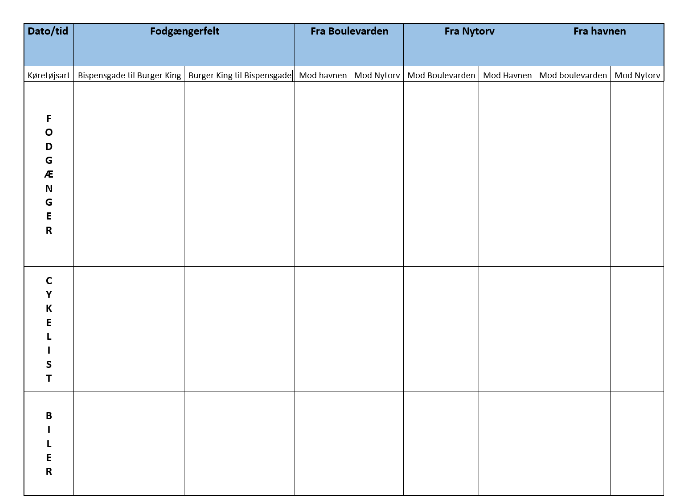
\includegraphics[scale=0.6]{figures/Billederogfigur/tabelp.png}
     \end{adjustbox}
      \caption{Tælleskema for trafiktællinger}
      \label{fig:tft}
    \end{figure}
